\documentclass[pdflatex,compress]{beamer}

%\usetheme[dark,framenumber,totalframenumber]{ElektroITK}
\usetheme[darktitle,framenumber,totalframenumber]{ElektroITK}
\usepackage{graphicx}
\usepackage{multicol}

\title{Data Communications}
\subtitle{Chapter 6 - Error Detection and Correction}

\author{Mifta Nur Farid}

\begin{document}

\maketitle

\begin{frame}
	\frametitle{Types of Errors}
	\begin{itemize}
		\item An error occurs when a bit is altered between transmission and reception
		\begin{itemize}
			\item Binary 1 is transmitted and binary 0 is received
			\item Binary 0 is transmitted and binary 1 is received
		\end{itemize}
		\item \textbf{Single bit errors}
		\begin{itemize}
			\item Isolated error that alters one bit but does not affect nearby bits
			\item Can occur in the presence of white noise
		\end{itemize}
		\item \textbf{Burst errors}
		\begin{itemize}
			\item Contiguous sequence of B bits in which the first and last bits and any number of intermediate bits are received in error
			\item Can be caused by impulse noise or by fading in a mobile wireless environment
			\item Effects of burst errors are greater at higher data rates
		\end{itemize}
	\end{itemize}
\end{frame}

\begin{frame}
	\frametitle{Burst and Single-Bit Errors}
	\begin{center}
		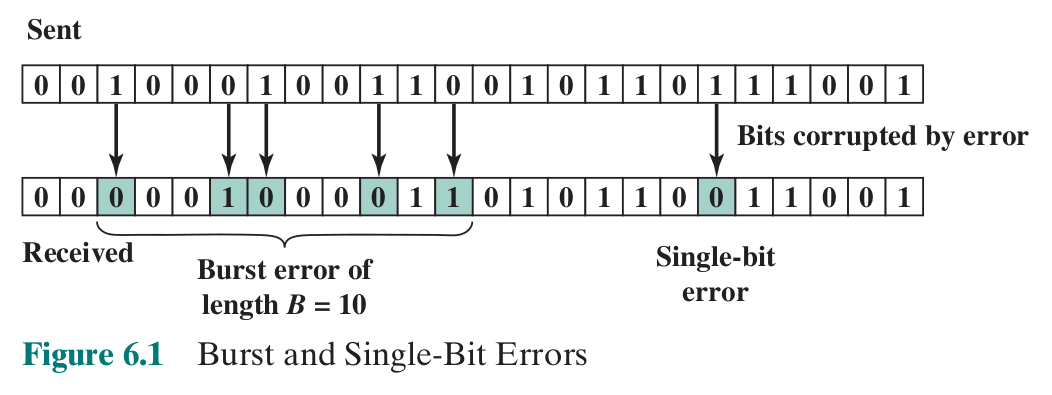
\includegraphics[width=\linewidth]{img/img01}
	\end{center}
\end{frame}

\begin{frame}
	\frametitle{Error Detection}
	\begin{itemize}
		\item Regardless of design you will have errors, resulting in the change of one or more bits in a transmitted frame
		\item Frames
		\begin{itemize}
			\item Data transmitted as one or more contiguous sequences of bits
			\item[$ P_b $ :] Probability that a bit is received in error; also known as the bit error rate (BER)
			\item[$ P_1 $ :] Probability that a frame arrives with no bit errors
			\item[$ P_2 $ :] Probability that, with an error-detecting algorithm in use, a frame arrives with one or more undetected errors
			\item[$ P_3 $ :] Probability that, with an error-detecting algorithm in use, a frame arrives with one or more detected bit errors but no undetected bit errors
		\end{itemize}
	\end{itemize}
\end{frame}

\begin{frame}{Error Detection}
	\begin{itemize}
		\item The probability that a frame arrives with no bit errors decreases when the probability of a single bit error increases
		\item The probability that a frame arrives with no bit errors decreases with increasing frame length
		\begin{itemize}
			\item The longer the frame, the more bits it has and the higher the probability that one of these is in error
		\end{itemize}
	\end{itemize}
\end{frame}

\begin{frame}
	\frametitle{Error Detection Process}
	\begin{center}
		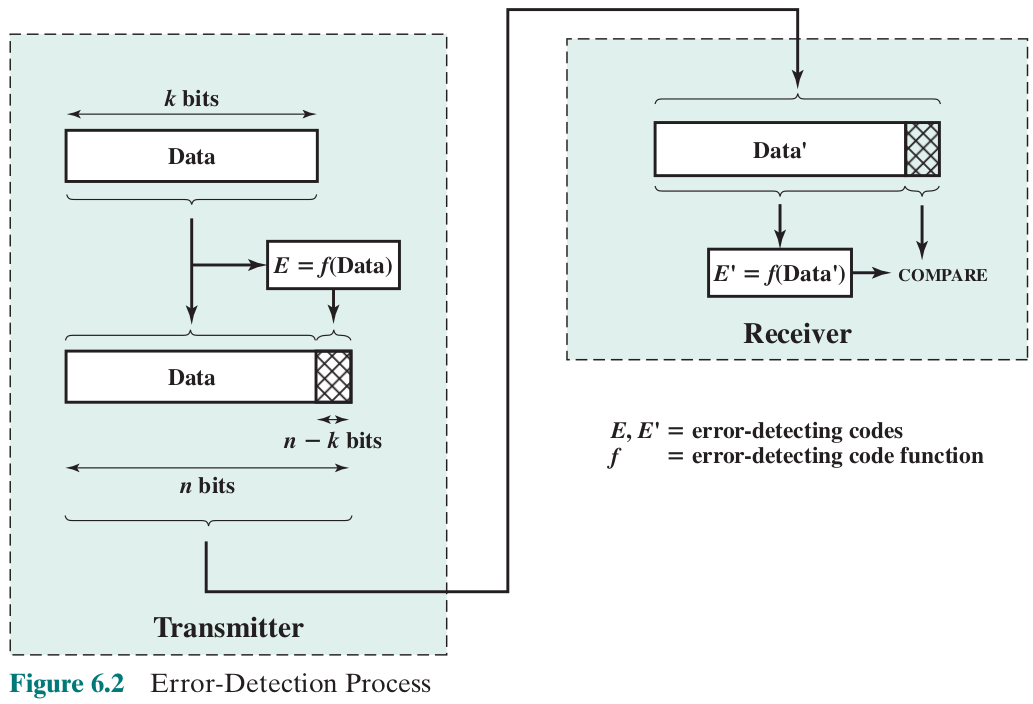
\includegraphics[width=\linewidth]{img/img02}
	\end{center}
\end{frame}

\begin{frame}
	\frametitle{Parity Check}
	\begin{itemize}
		\item The simplest error detecting scheme is to append a parity bit to the end of a block of data
		\begin{itemize}
			\item Even Parity
			\begin{itemize}
				\item Even number of 1s
				\item Used for synchronous transmission
			\end{itemize}
			\item Odd Parity
			\begin{itemize}
				\item Odd number of 1s
				\item Used for asynchronous transmission
			\end{itemize}
		\end{itemize}
		\item If any even number of bits are inverted due to error, an undetected error occurs
	\end{itemize}
\end{frame}

\end{document}
